% Choose one to switch between slides and handout
%\documentclass[]{beamer}
\documentclass[handout]{beamer}

% Video Meta Data
\title{Bitcoin, Blockchain and Cryptoassets}
\subtitle{CBDC and Stablecoins}
\author{Prof. Dr. Fabian Schär}
\institute{University of Basel}

% Config File
% Packages
\usepackage[utf8]{inputenc}
\usepackage{hyperref}
\usepackage{gitinfo2}
\usepackage{tikz}
\usepackage{amsmath}
\usepackage{mathtools}
\usepackage{bibentry}
\usepackage{xcolor}
\usepackage{colortbl} % Add colour to LaTeX tables
\usepackage{caption}
\usepackage[export]{adjustbox}
\usepackage{pgfplots} \pgfplotsset{compat = 1.17}
\usepackage{makecell}
\usepackage{fancybox}
\usepackage{ragged2e}
\usepackage{fontawesome}
\usepackage{seqsplit}
\usepackage{tabularx}

% Color Options
\definecolor{highlight}{rgb}{0.65,0.84,0.82}
\definecolor{focus}{rgb}{0.72, 0, 0}
\definecolor{lightred}{rgb}{0.8,0.5,0.5}
\definecolor{midgray}{RGB}{190,195,200}

% Beamer Template Options
\beamertemplatenavigationsymbolsempty
\setbeamertemplate{footline}[frame number]
\setbeamercolor{structure}{fg=black}
\setbeamercolor{footline}{fg=black}
\setbeamercolor{title}{fg=black}
\setbeamercolor{frametitle}{fg=black}
\setbeamercolor{item}{fg=black}
\setbeamercolor{}{fg=black}
\setbeamercolor{bibliography item}{fg=black}
\setbeamercolor*{bibliography entry title}{fg=black}
\setbeamercolor{alerted text}{fg=focus}
\setbeamertemplate{items}[square]
\setbeamertemplate{enumerate items}[default]
\captionsetup[figure]{labelfont={color=black},font={color=black}}
\captionsetup[table]{labelfont={color=black},font={color=black}}

\setbeamertemplate{bibliography item}{\insertbiblabel}

% Link Icon Command
\newcommand{\link}{%
    \tikz[x=1.2ex, y=1.2ex, baseline=-0.05ex]{%
        \begin{scope}[x=1ex, y=1ex]
            \clip (-0.1,-0.1)
                --++ (-0, 1.2)
                --++ (0.6, 0)
                --++ (0, -0.6)
                --++ (0.6, 0)
                --++ (0, -1);
            \path[draw,
                line width = 0.5,
                rounded corners=0.5]
                (0,0) rectangle (1,1);
        \end{scope}
        \path[draw, line width = 0.5] (0.5, 0.5)
            -- (1, 1);
        \path[draw, line width = 0.5] (0.6, 1)
            -- (1, 1) -- (1, 0.6);
        }
    }

% Read Git Data from Github Actions Workflow
% Defaults to gitinfo2 for local builds
\IfFileExists{gitInfo.txt}
	{\input{gitInfo.txt}}
	{
		\newcommand{\gitRelease}{(Local Release)}
		\newcommand{\gitSHA}{\gitHash}
		\newcommand{\gitDate}{\gitAuthorIsoDate}
	}

% Custom Titlepage
\defbeamertemplate*{title page}{customized}[1][]
{
  \vspace{-0cm}\hfill\includegraphics[width=2.5cm]{../config/logo_cif}
  \includegraphics[width=1.9cm]{../config/seal_wwz}
  \\ \vspace{2em}
  \usebeamerfont{title}\textbf{\inserttitle}\par
  \usebeamerfont{title}\usebeamercolor[fg]{title}\insertsubtitle\par  \vspace{1.5em}
  \small\usebeamerfont{author}\insertauthor\par
  \usebeamerfont{author}\insertinstitute\par \vspace{2em}
  \usebeamercolor[fg]{titlegraphic}\inserttitlegraphic
    \tiny \noindent \texttt{Release Ver.: \gitRelease}\\ 
    \texttt{Version Hash: \gitSHA}\\
    \texttt{Version Date: \gitDate}\\ \vspace{1em}
    
    
    \iffalse
  \link \href{https://github.com/cifunibas/Bitcoin-Blockchain-Cryptoassets/blob/main/slides/intro.pdf}
  {Get most recent version}\\
  \link \href{https://github.com/cifunibas/Bitcoin-Blockchain-Cryptoassets/blob/main/slides/intro.pdf}
  {Watch video lecture}\\ 
  
  \fi
  
  \vspace{1em}
  License: \texttt{Creative Commons Attribution-NonCommercial-ShareAlike 4.0 International}\\\vspace{2em}
  \includegraphics[width = 1.2cm]{../config/license}
}


% tikzlibraries
\usetikzlibrary{decorations.pathreplacing}
\usetikzlibrary{decorations.markings}
\usetikzlibrary{positioning}
\usetikzlibrary{calc}
\captionsetup{font=footnotesize}


%%%%%%%%%%%%%%%%%%%%%%%%%%%%%%%%%%%%%%%%%%%%%%
%%%%%%%%%%%%%%%%%%%%%%%%%%%%%%%%%%%%%%%%%%%%%%
\begin{document}

\thispagestyle{empty}
\begin{frame}[noframenumbering]
	\titlepage
\end{frame}

%%%

%%%
\begin{frame}{CBDC Background}

Established model of central banks as issuer of physical cash and lender of last resort.\\ \vspace{1em}

 But: General public can only hold legal tender in the form of cash. No access to Central Bank ledger. This may change.
\vspace{1.5em}	

\textbf{Important Factors:}
\begin{itemize}
	\item \textbf{Drop in physical cash use} and growing importance of digital payment systems as essential infrastructure.
	\item \textbf{Emergence of new payment solutions} from private sector, with large actors outside the banking industry.
	\item \textbf{Ongoing debate on mandate} of central banks around money issuance and payment infrastructure provision.
\end{itemize}

\end{frame}
%%%

%%%

\begin{frame}{CBDC Overview}
CBDC as any \color{focus} digital form of money issued by a central bank. \color{black} 

\begin{center}
	\begin{tikzpicture}[scale=0.4, every node/.style ={scale=0.8}]
		\begin{tikzpicture}[scale = 0.7, every node/.style={scale=0.85}]

	\draw[color=black, ->] (0,0) -- (6,-1);
    \draw[color=black] plot (3,-0.5) node[color=black,below, rotate = -9] {\scriptsize{\textbf{Representation}}};
    
     \draw[color=black, ->] (0,0) -- (0,5);
     \draw[color=black] plot (0,2.5) node[color=black,above, rotate = 90] {\scriptsize{\textbf{Transaction processing}}};
     
     \draw[color=black, ->] (0,0) -- (5,1.5);
     \draw[color=black] plot (2.5,0.75) node[color=black, above, rotate = 17] {\scriptsize{\textbf{Creation}}};
     
     \draw[color=black, dotted] (0,5) -- (6, 4);
     \draw[color=focus, thick, dotted] (6,-1) -- (6, 4);
     \draw[color=black, dotted] (5,1.5) -- (11, 0.5);
     \draw[color=black, dotted] (0,5) -- (5, 6.5);
     \draw[color=black, dotted] (5,1.5) -- (5, 6.5);
     \draw[color=black, dotted] (5,6.5) -- (11, 5.5);
     \draw[color=black, dotted] (11,0.5) -- (11, 5.5);
     \draw[color=black, dotted] (6,-1) -- (11, 0.5);
     \draw[color=black, dotted] (6,4) -- (11, 5.5);
     
	\draw 	(0,5) circle (0.12cm) node[right,color=black] {\scriptsize{Cash}};
     
    \draw	(5,6.5) circle (0.12cm) node[right,color=black] {\scriptsize{Commodity money}};
     
    \draw	(11,0.5) circle (0.12cm) node[right,color=black] {\scriptsize{Comm.\ bank deposits}};
     
	\draw	(11,5.5) circle (0.12cm) node[right,color=black] {\scriptsize{Bitcoin}};

     \draw[color=black] plot (0,0) node[left, rotate = 0] {\tiny{centralized}};
     \draw[color=black] plot (0,5) node[left, rotate = 0] {\tiny{decentralized}};
     
     \draw[color=focus] plot (0.5,0.2) node[right, rotate = 90] {\tiny{monopolistic}};
     \draw[color=black] plot (4.45,3.1) node[left, rotate = 90] {\tiny{competitive}};
          
     \draw[color=black] plot (0.85,-0.19) node[below, rotate = -9] {\tiny{physical}};
     \draw[color=focus] plot (5.1,-0.9) node[below, rotate = -9] {\tiny{virtual}};
     
\end{tikzpicture}
	\end{tikzpicture}
\end{center}


\uncover<2->{
Selected CBDC design dimensions:
	\begin{itemize}
		\item Centralized vs. decentralized
		\item Retail vs. wholesale
		\item Token-/Object- vs. Account-based
	\end{itemize}
}

\end{frame}
%%%

%%%
\begin{frame}{CBDC Status and Arguments}

\begin{itemize}
	\item Research in the area of e-money/e-cash since the 1990s.
	\item Various pilots since 2014.\\
			\textit{E.g., Dinero Electronico, eKrona, project Jasper, digital yuan.}
	\item Becoming increasingly more important with a large variety of pilots all around the world: \link{\href{https://cbdctracker.org}{Infopage: cbdctracker.org}}
\end{itemize}

\vspace{1.0em}

\uncover<2->{
\begin{columns}[T]
	\begin{column}{0.2\textwidth}
		\textbf{Proponents}
	\end{column}
	\begin{column}{0.1\textwidth}
		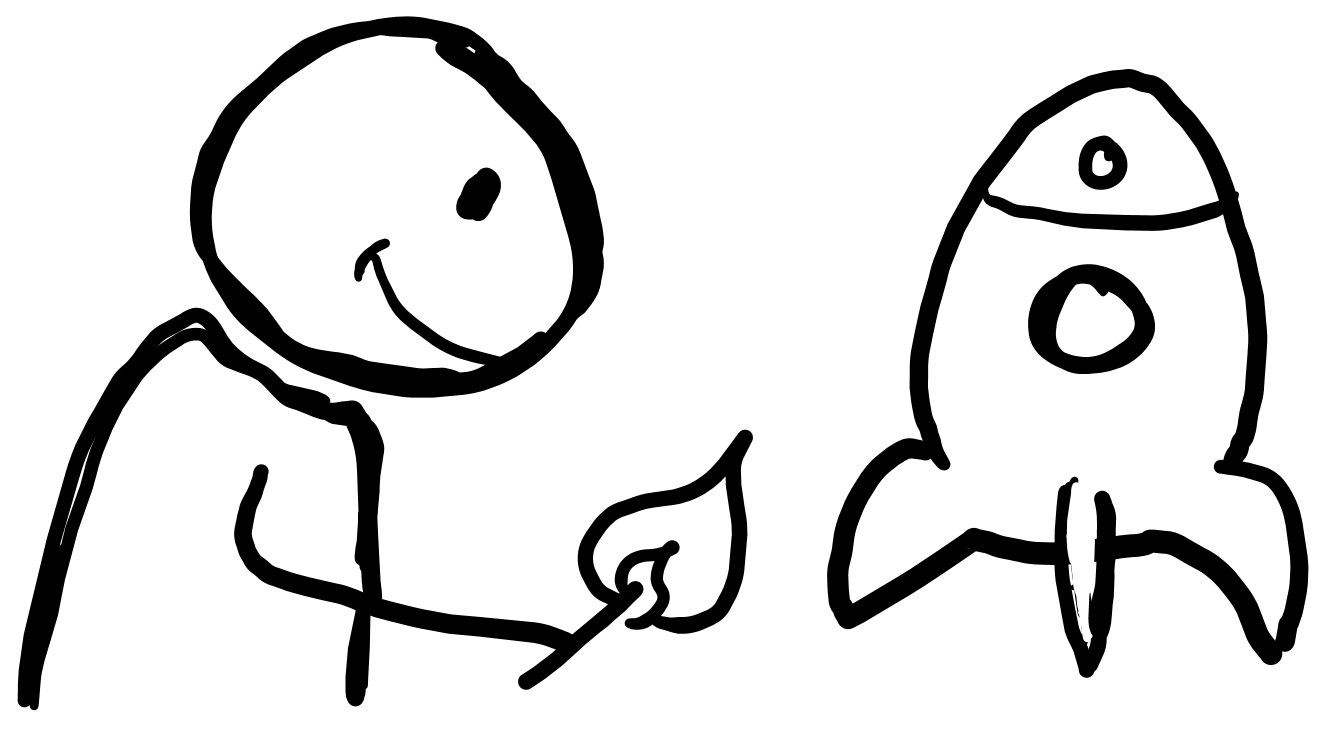
\includegraphics[height = 0.9cm]{../assets/images/agents/proponent}
	\end{column} %\hfill
	\begin{column}{0.2\textwidth}
		\textbf{Critics}
	\end{column}
	\begin{column}{0.1\textwidth}
		
\includegraphics[height = 1cm]{../assets/images/agents/opponent}
	\end{column} %\hfill
\end{columns}

\vspace{0.5em}

\begin{columns}[T]
	\begin{column}{0.45\textwidth}
	\footnotesize{
		\begin{itemize}
			\item Enhanced transmission of monetary policy
			\item Mitigation of incentivisation issues in the banking sector
			\item Potential in counteracting money-laundering
		\end{itemize}
		}
	\end{column}
	\begin{column}{0.45\textwidth}
	\footnotesize{
		\begin{itemize}
			\item Undesired structural disintermediation of banks 
			\item Unknown effects on financial stability
			\item Privacy concerns and severe centralization risks
		\end{itemize}
		}
	\end{column}
\end{columns}
}

\end{frame}
%%%

%%%
\begin{frame}{Stablecoins Overview}
A privately issued cryptoasset that is \color{focus} pegged to another asset \color{black} (usually a FIAT currency) with the goal to decrease price volatility and create a Blockchain-based medium of exchange. 

\vspace{1.5em}

\uncover<2->{
\textbf{Three main categories:}
	\begin{itemize}
		\item<2-> Off-chain collateralized
		\begin{itemize}
			\item<2-> Examples: \textit{USDT, TUSD, USDC}
			\item<2-> Risks: counterparty risk, regulatory risk.
		\end{itemize}
		\item<3-> On-chain collateralized\\
		\begin{itemize}
			\item<3-> Examples: \textit{DAI, sUSD}
			\item<3-> Risks: liquidation risk, smart contract risk, oracle risk.
		\end{itemize}
		\item<4-> Algorithmic stablecoin\\
		\begin{itemize}
			\item<4-> Examples: \textit{...}
			\item<4-> Risks: Flawed economics.
		\end{itemize}
	\end{itemize}
}

\end{frame}
%%%

%%%
\begin{frame}{References and Recommended Reading}
		\begin{columns}[T]
			\begin{column}{0.1\textwidth}
					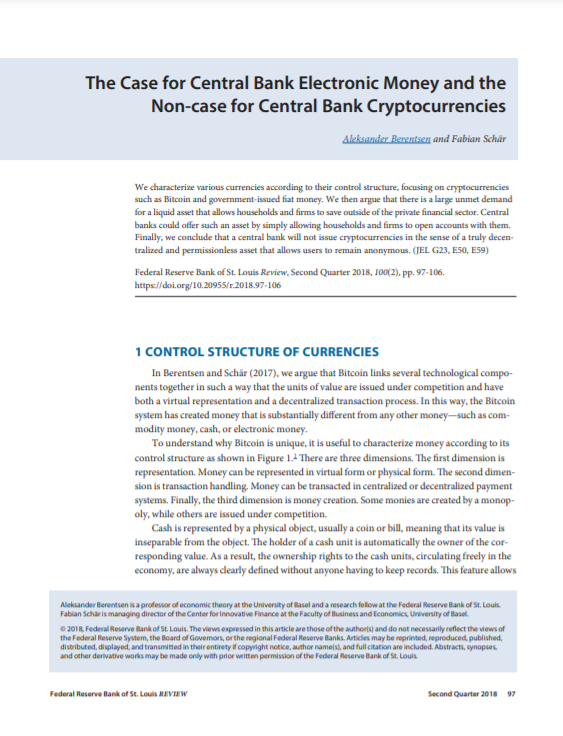
\includegraphics[width = 1.7cm, frame]{../assets/images/berentsen_schaer}
			\end{column} %\hfill
			\begin{column}{0.8\textwidth}
				\textbf{The Case for Central Bank Electronic Money and the Non-case for Central Bank Cryptocurrencies} \\ 
				Aleksander Berentsen and Fabian Schär \\
				\link \href{https://research.stlouisfed.org/publications/review/2018/02/13/the-case-for-central-bank-electronic-money-and-the-non-case-for-central-bank-cryptocurrencies}{Online version}
			\end{column}
		\end{columns}
	
\end{frame}
%%%

\end{document}
